\documentclass[16pts]{report}
\usepackage[utf8]{inputenc}
\usepackage[T1]{fontenc}
\usepackage[francais]{babel}
\usepackage{xcolor}
\usepackage[hyphens]{url}
\usepackage[hidelinks]{hyperref}
\usepackage{amsmath}
\usepackage{graphicx}
\usepackage{geometry}
\usepackage{textcomp}
\hypersetup{hypertexnames=true}
\geometry{hmargin=2.5cm,vmargin=1.5cm}

\usepackage{float} %Option H pour les figures, utile.

%\maketitle
%\clearpage

\begin{document}
\bibliographystyle{unsrt}
\nocite{*}

\chapter{Évolutions}
\label{cha:Evolutions}

\section{Évolution des besoins}
\label{sec:Evolution des besoins}

Durant la phase de conception de notre projet, nous nous sommes confrontés à 
deux difficultés qui ont fait évoluer nos besoins. En effet, nos recherches 
nous pas permis de pouvoir résoudre les conflits automatiquement ni de générer 
une configuration par défaut en fonction du matériel de l'utilisateur, comme
cela a été évoqué précédemment. 
\\
L'objectif de résolution automatique des conflits a été modifié afin de 
simplement aider l'utilisateur à trouver les conflits d'une option. Il se 
chargera de modifier les valeurs des options par lui-même.
\\
En ce qui concerne le besoin de détecter le matériel d'un utilisateur, celui-ci 
s'est transformé pour devenir une base de données communautaire. Celle-ci est 
modifiable à l'aide d'un site web. Il est possible d'ajouter des relations 
entre des options et des modules, et entre des modules et du matériel. Les 
modules représentent la partie Driver. Un second besoin était de pouvoir 
ajouter des Tags aux options afin de pouvoir les regrouper afin d'affiner la 
recherche. Ce besoin a également été ajouté sur cette base communautaire.

\begin{figure}[H]
	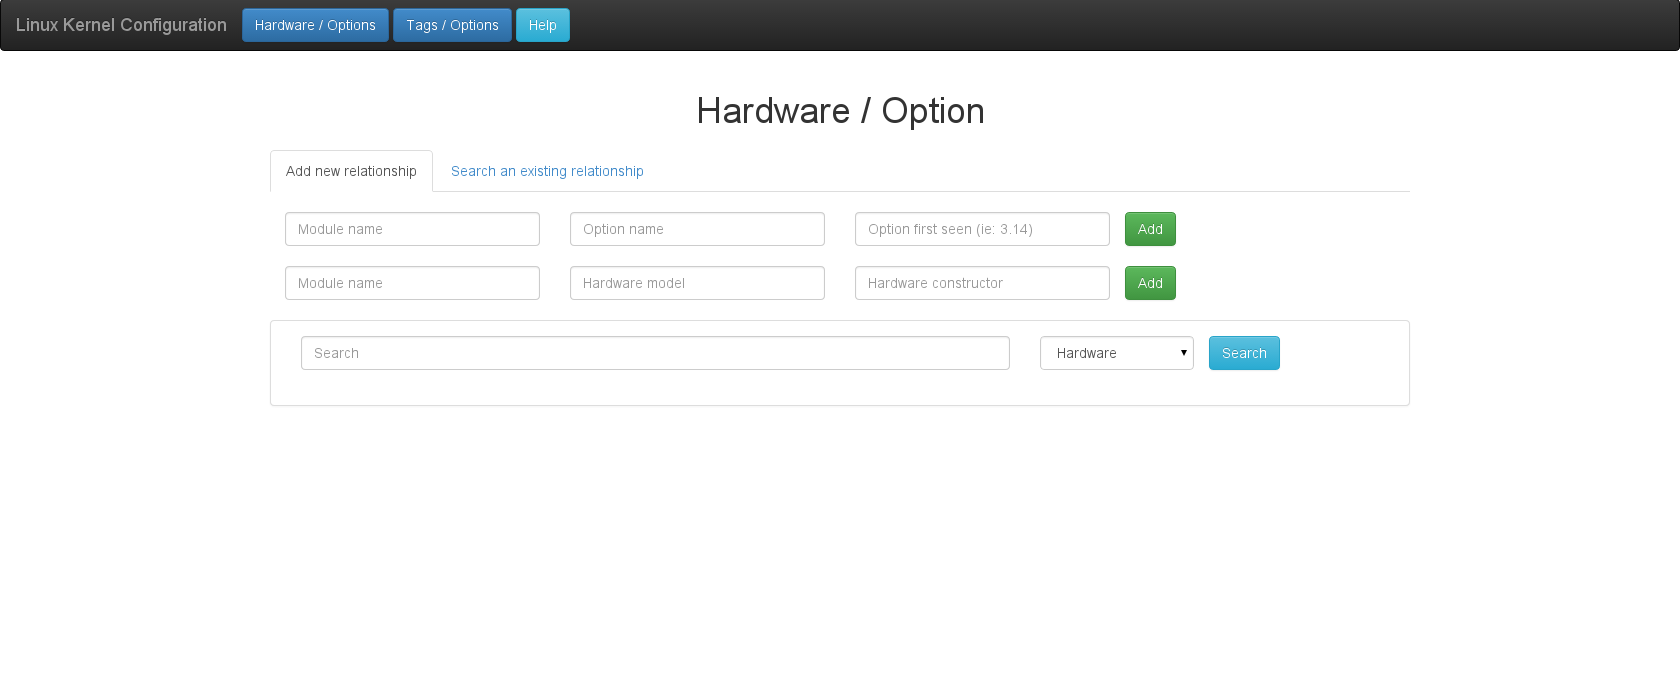
\includegraphics[scale=0.3]{../illustrations/screen_site_hardware.png}
	\centering
	\caption{Diagramme des classes du site}
	\label{fig:DiagSite}
\end{figure}

\begin{figure}[H]
	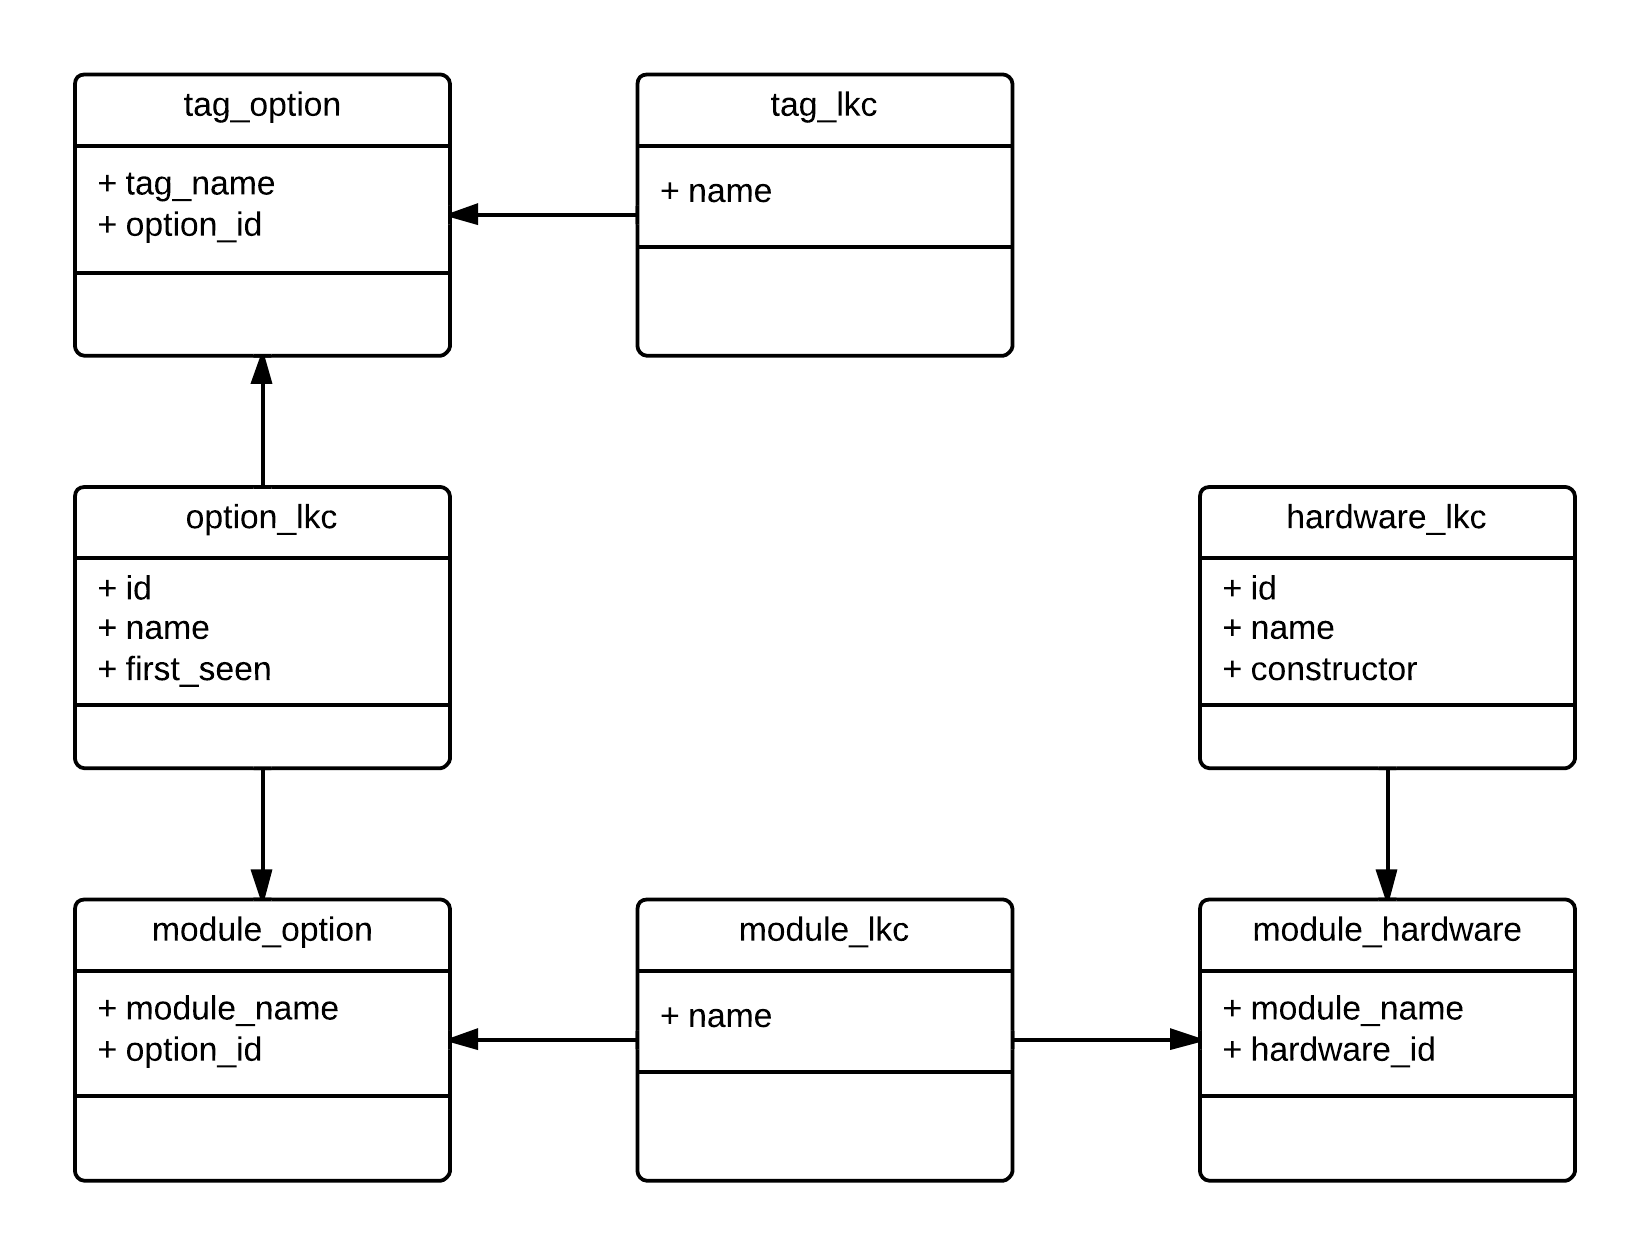
\includegraphics[scale=0.2]{../illustrations/diagramme_classes_site.png}
	\centering
	\caption{Diagramme des classes du site}
	\label{fig:DiagSite}
\end{figure}

(On verra quand le site aura avancé)

\pagebreak

\section{Évolution de l'interface}
\label{sec:Evolution de l'interface}

En parallèle de l'évolution des besoins, l'ergonomie de l'interface a changé 
afin d'améliorer l'utilisation de l'application et afin de correspondre aux 
fonctionnalités attendues.

\begin{enumerate}

	\item Évolution de l'interface de configuration de l'application
	\\

	L'interface de configuration permet à l'utilisateur de choisir le noyau 
	et l'architecture qu'il désire. Il peut également charger un fichier de 
	configuration existant.

	\begin{figure}[H]
		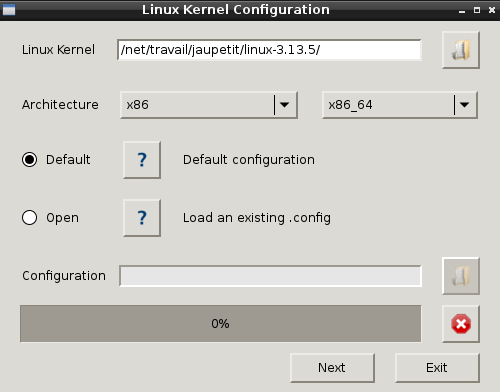
\includegraphics[scale=0.7]{../illustrations/screen_configuration_interface.png}
		\centering
		\caption{Évolution de l'interface de configuration de l'application}
		\label{fig:Evo_config}
	\end{figure}

	L'utilisateur n'a plus que deux choix contre quatre auparavant. En effet, 
	il ne peut plus détecter son matériel automatiquement comme cela était 
	le cas sur les maquettes. Il ne peut plus créer une configuration vierge, 
	car certaines options sont nécessaires pour ne pas créer de conflits.
	\\

	\pagebreak	

	\item Évolution de l'interface d'affichage des options
	\\

	L'interface de modification des options autorise l'utilisateur à naviguer 
	entre les options avec différents menus. Il peut modifier leurs valeurs 
	s'il n'y a pas de conflit et générer un fichier de configuration lorsqu'il 
	a terminé.

	\begin{figure}[H]
		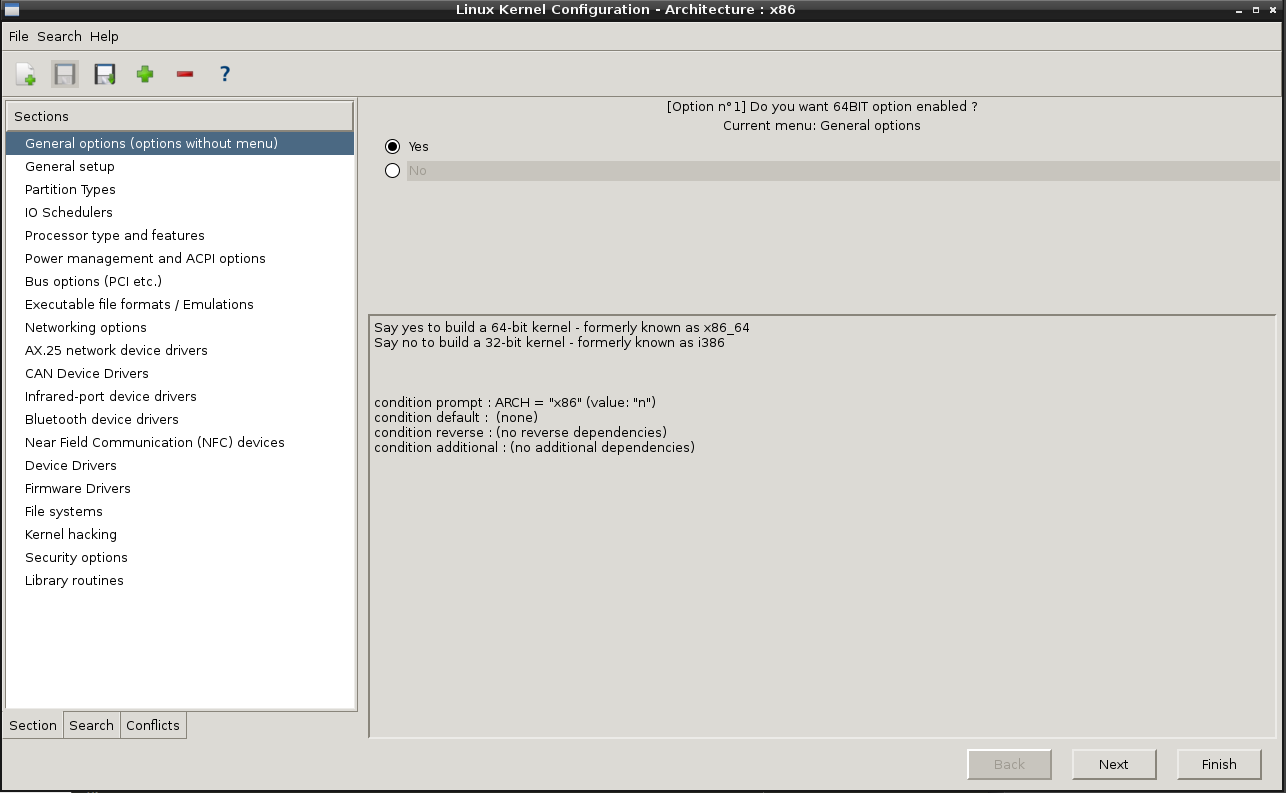
\includegraphics[scale=0.5]{../illustrations/screen_options_interface.png}
		\centering
		\caption{Évolution de l'interface d'affichage des options}
		\label{fig:Evo_config}
	\end{figure}

	Lorsqu'une option est sélectionnée, il n'y a plus seulement sa description d'affiché, mais également ses dépendances. Cela permet à l'utilisateur de 
	pouvoir corriger d'éventuels conflits plus facilement.

	\pagebreak	

	\item Évolution de l'interface de recherche des options
	\\

	L'onglet \"Search\" permet à l'utilisateur d'afficher la liste complète 
	des options sous la forme d'un arbre ou une liste plus réduite en 
	saisissant une chaine à rechercher.

	\begin{figure}[H]
		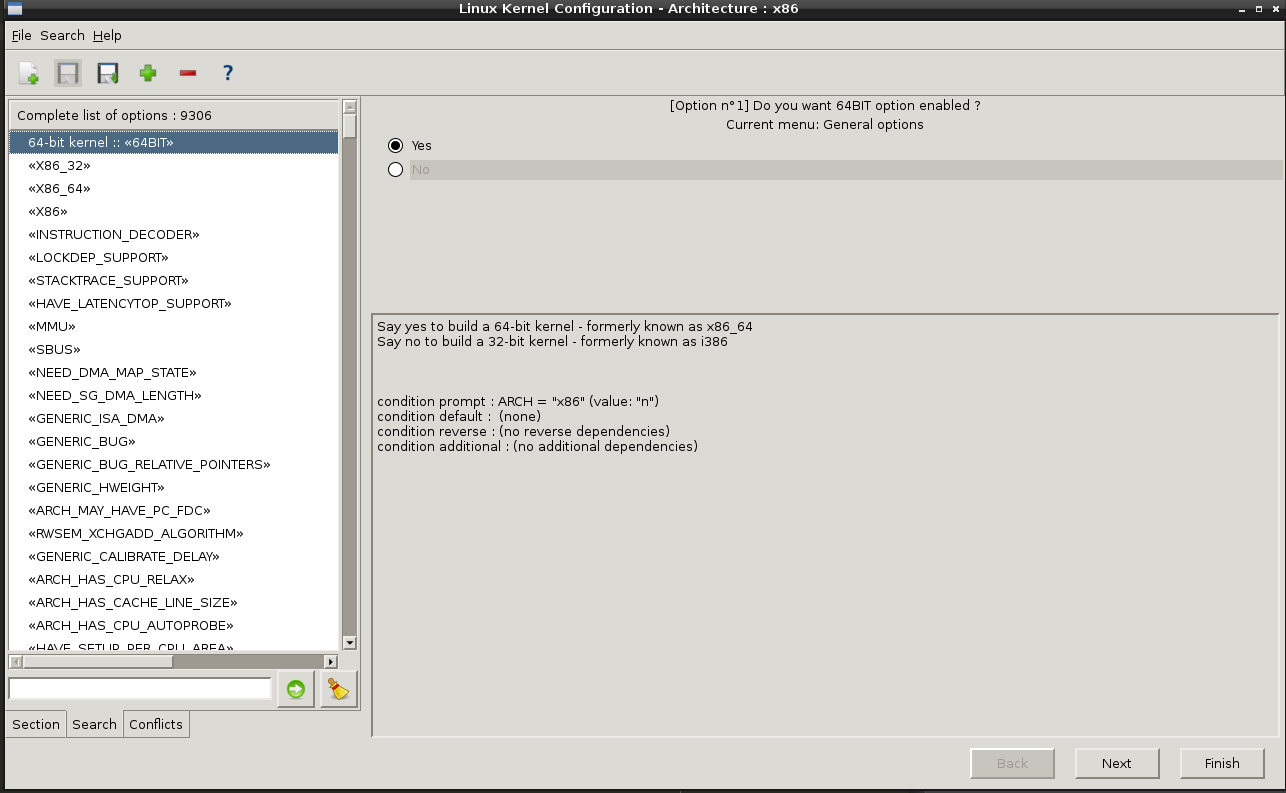
\includegraphics[scale=0.5]{../illustrations/screen_options_search_interface.png}
		\centering
		\caption{Évolution de l'interface de recherche des options}
		\label{fig:Evo_config}
	\end{figure}

	Dans les outils existants ainsi que dans les premiers prototypes, il est seulement possible de faire une recherche sur les noms des options. 
	Dorénavant, l'utilisateur peut cliquer le menu \"Search\" en haut de la 
	fenêtre pour sélectionner où il souhaite rechercher. Il peut chercher dans 
	les noms, les descriptions et les aides des options.
	\\

	\pagebreak	

	\item Évolution de l'interface d'affichage des conflits
	\\

	À l'origine, il y avait un bouton sur l'interface permettant d'ouvrir 
	une fenêtre pour résoudre les conflits. Il y avait un second bouton relatif 
	à l'ajout de Tags. Il a également disparu, car les tags sont uniquement 
	gérés par un site. 

	*** (FIXME VERIFIER que l'on a évoqué le site auparavant)

	\begin{figure}[H]
		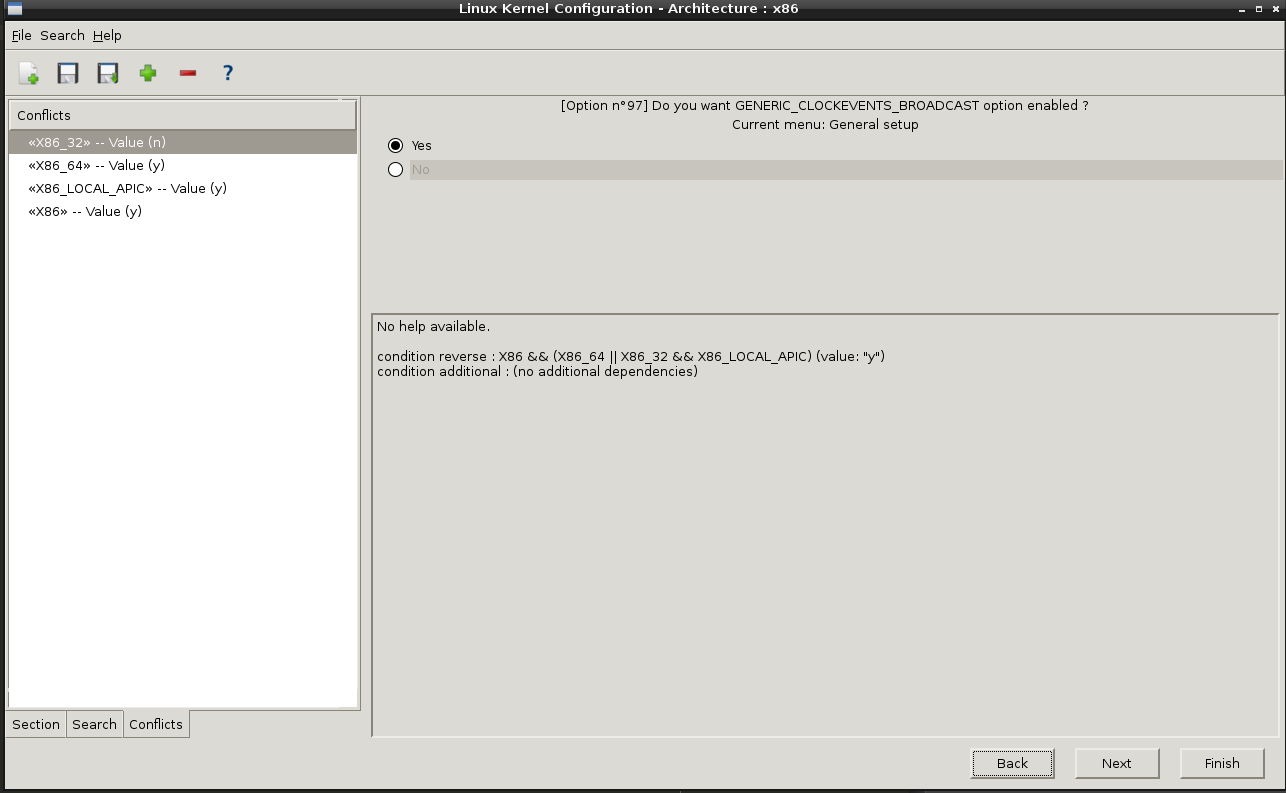
\includegraphics[scale=0.5]{../illustrations/screen_options_conflits_interface.png}
		\centering
		\caption{Évolution de l'interface d'affichage des conflits}
		\label{fig:Evo_config}
	\end{figure}

	Un nouvel onglet est apparu à droite de la recherche. L'idée de résoudre 
	les conflits automatiquement a été remplacée par cet onglet. Il affiche 
	la liste des options en conflit avec l'option courante. Cela permet à 
	l'utilisateur de se positionner rapidement sur les options qui posent 
	problème. 
	\\



\end{enumerate}

\end{document}
